\chapter{Regulacja DMC}
\section{Algorytm i testy}
Zaprojektowano analityczny regulator DMC na podstawie odpowiedzi skokowej modelu liniowego. W każdej próbce algorytm wyznacza przyszłe przyrosty sterowania minimalizujące błąd predykcji wyjścia i zmiany sterowania, a na obiekt podaje tylko pierwszy z nich. Dzięki uwzględnieniu historii sterowań regulator dobrze radzi sobie z opóźnieniem transportowym $200\ \mathrm{s}$. Przyjęto nastawy: $D=250$, $N=50$, $N_u=10$, $\lambda=\num{0.05}$ oraz $T_s=20\ \mathrm{s}$. Regulator działa bez ograniczeń, a zakłócenie $F_D$ tłumi przez sprzężenie zwrotne.

Na obu obiektach w $400\ \mathrm{s}$ zmieniano zadany poziom, a w $3800\ \mathrm{s}$ zakłócenie. Dla każdej próby pokazano wyjście $y(k)=h_2(k)$ i sterowanie $u(k)=\uvar(k)$ na wspólnej osi czasu.
\begin{figure}[H]
\centering
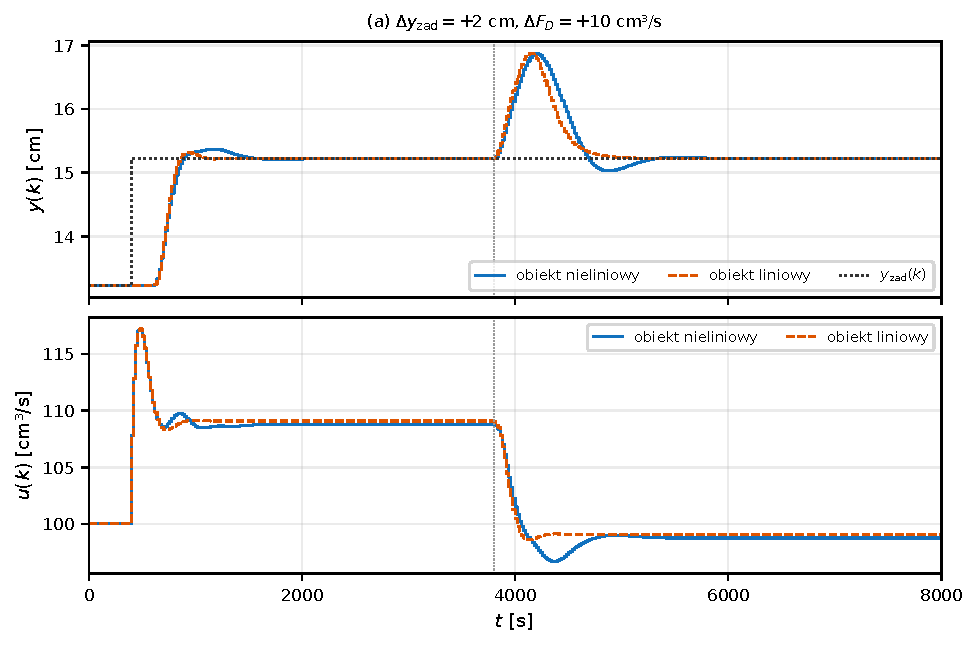
\includegraphics[width=0.94\textwidth]{rysunki/czesc1/DMC_scenariusz_1.pdf}
\caption{Próba 1: $\Delta y_{\mathrm{zad}}=+2\ \mathrm{cm}$, $\Delta F_D=+10\ \jednprzep$. Wyjście $y(k)$ i bezpośrednio pod nim sterowanie $u(k)$; pionowa linia oznacza skok $F_D$.}
\label{fig:dmcY}
\end{figure}
Dla małych skoków przebiegi obu obiektów są zbliżone, zarówno dla wyjścia, jak i sterowania.

\clearpage
\section{Skok zadania o 4 cm}
Po dodatnim skoku zakłócenia regulator zmniejsza dopływ. Skutek korekcji dociera do obiektu po czasie transportu, dlatego poziom przejściowo rośnie.
\begin{figure}[H]
\centering
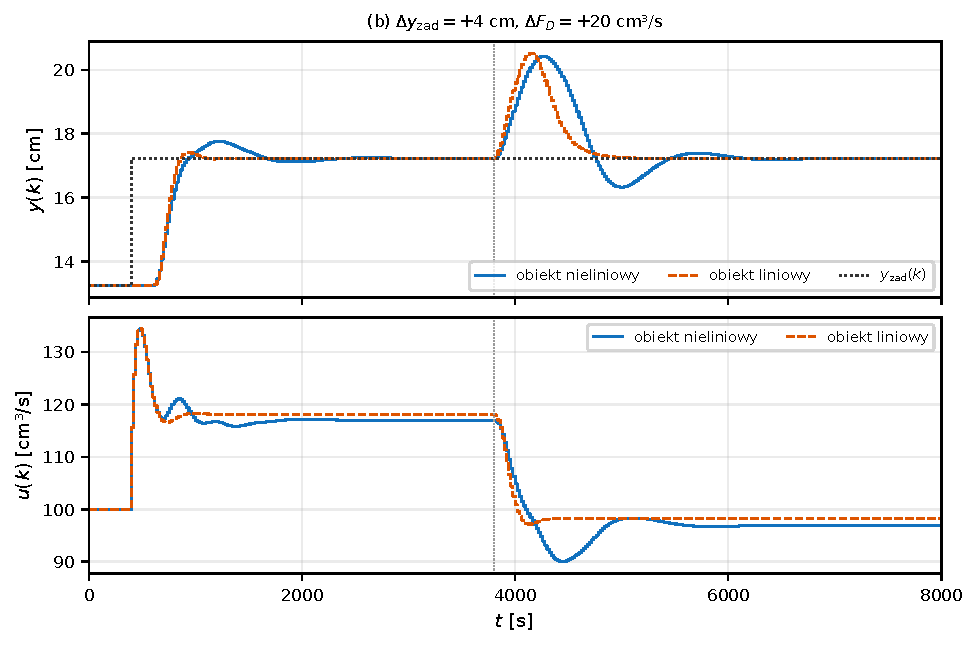
\includegraphics[width=0.94\textwidth]{rysunki/czesc1/DMC_scenariusz_2.pdf}
\caption{Próba 2: $\Delta y_{\mathrm{zad}}=+4\ \mathrm{cm}$, $\Delta F_D=+20\ \jednprzep$. Wyjście i sterowanie na wspólnej osi czasu.}
\label{fig:dmcU}
\end{figure}

\clearpage
\section{Duży dodatni skok zadania}
\begin{figure}[H]
\centering
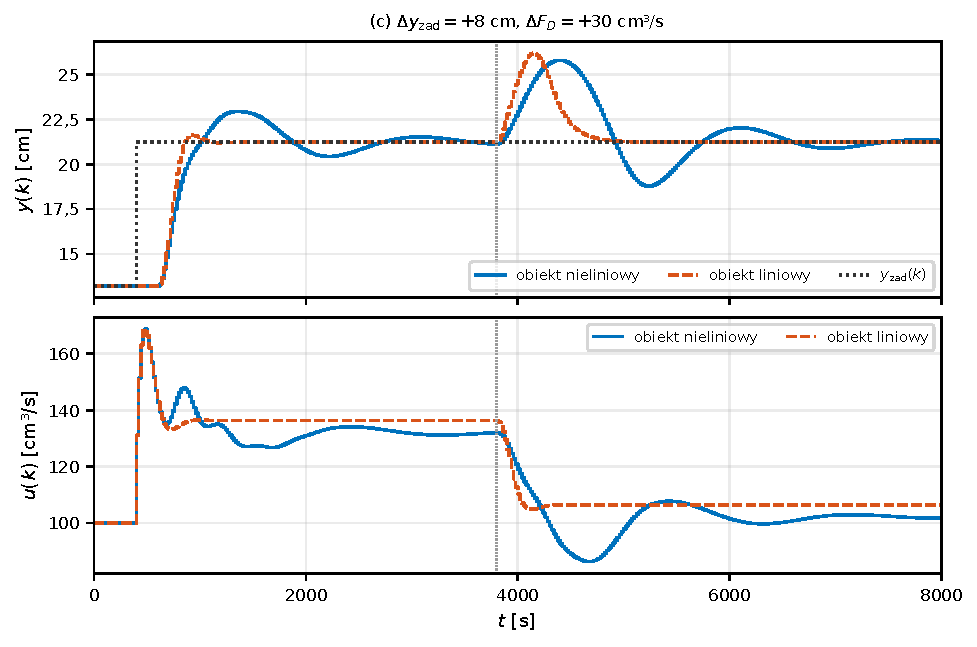
\includegraphics[width=\textwidth]{rysunki/czesc1/DMC_scenariusz_3.pdf}
\caption{Próba 3: $\Delta y_{\mathrm{zad}}=+8\ \mathrm{cm}$, $\Delta F_D=+30\ \jednprzep$. Wyjście $y(k)$ oraz odpowiadające mu sterowanie $u(k)$.}
\label{fig:dmc4}
\end{figure}
Przy dużym dodatnim skoku obiekt nieliniowy silniej oscyluje. Widać również większe korekty sterowania niż dla obiektu liniowego. Maksymalna różnica wyjść sięga $\num{3.37}\ \mathrm{cm}$.

\clearpage
\section{Duży ujemny skok zadania}
\begin{figure}[H]
\centering
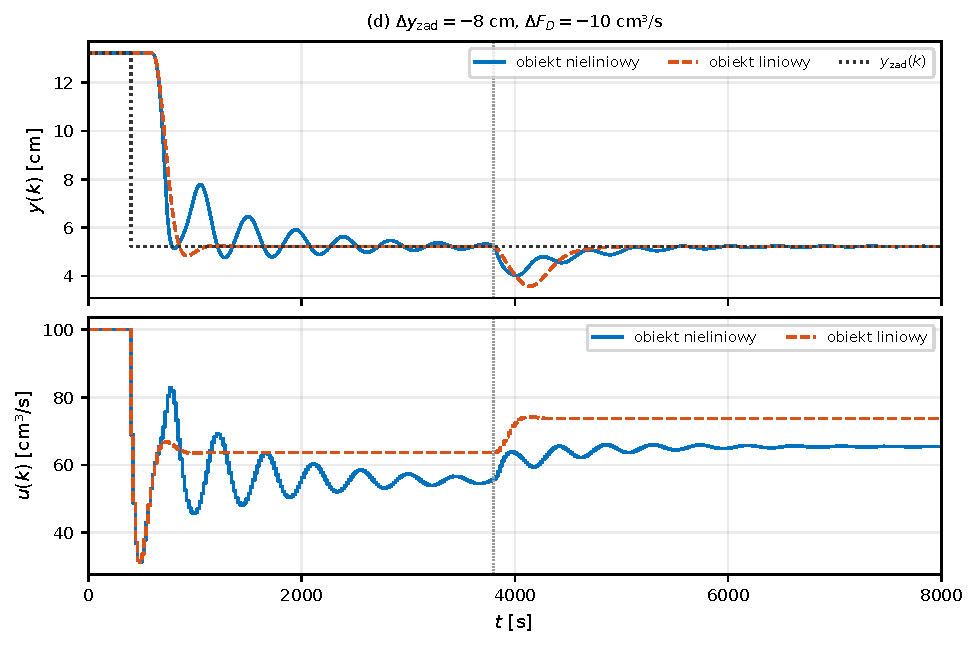
\includegraphics[width=\textwidth]{rysunki/czesc1/DMC_scenariusz_4.pdf}
\caption{Próba 4: $\Delta y_{\mathrm{zad}}=-8\ \mathrm{cm}$, $\Delta F_D=-10\ \jednprzep$. Wyjście $y(k)$ i sterowanie $u(k)$.}
\label{fig:dmcUjemny}
\end{figure}
Obniżenie zadania wymaga zmniejszenia dopływu. Oscylacje poziomu na obiekcie nieliniowym wiążą się z oscylacjami sterowania. Minimalny dopływ to około $\num{31.19}\ \jednprzep$.

\clearpage
\section{Ocena jakości regulacji}
Uchyb regulacji to wartość zadana $y_{\mathrm{zad}}(k)$ minus zmierzony poziom $y(k)=h_2(k)$:
\begin{equation}
e(k)=y_{\mathrm{zad}}(k)-y(k).
\end{equation}
Jakość regulacji obiektu nieliniowego oceniono wskaźnikiem
\begin{equation}
\mathrm{IAE}=T_s\sum_k|y_{\mathrm{zad}}(k)-y(k)|=T_s\sum_k|e(k)|.
\end{equation}
Dla zadania sumowano próbki od $400$ do chwili poprzedzającej $3800\ \mathrm{s}$, a dla zakłócenia od $3800$ do $8000\ \mathrm{s}$.
\begin{table}[H]
\centering\small
\caption{Wyniki regulacji obiektu nieliniowego i różnica wyjść obu pętli}
\begin{tabular}{rrrrr}
\toprule
$\Delta y_{\mathrm{zad}}$ & $\Delta F_D$ & $\mathrm{IAE}_{\mathrm{zad}}$ & $\mathrm{IAE}_D$ & $\max|y_{\mathrm{NL}}-y_{\mathrm{L}}|$\\
{}[cm] & [$\jednprzep$] & [$\mathrm{cm\cdot s}$] & [$\mathrm{cm\cdot s}$] & [cm]\\
\midrule
\tableinput{dane/DMC_wskazniki.tex}
\bottomrule
\end{tabular}
\end{table}
W badanych próbach sterowanie pozostało dodatnie; najmniejsza wartość wynosiła około $\num{31.19}\ \jednprzep$. Przy większych skokach rosną oscylacje i rozbieżności modeli. W dodatnich scenariuszach zwiększano jednocześnie zmianę zadania i zakłócenia, dlatego sam wzrost IAE nie pozwala oddzielić wpływu tych dwóch czynników.
